\documentclass[1p]{elsarticle_modified}
%\bibliographystyle{elsarticle-num}

%\usepackage[colorlinks]{hyperref}
%\usepackage{abbrmath_seonhwa} %\Abb, \Ascr, \Acal ,\Abf, \Afrak
\usepackage{amsfonts}
\usepackage{amssymb}
\usepackage{amsmath}
\usepackage{amsthm}
\usepackage{scalefnt}
\usepackage{amsbsy}
\usepackage{kotex}
\usepackage{caption}
\usepackage{subfig}
\usepackage{color}
\usepackage{graphicx}
\usepackage{xcolor} %% white, black, red, green, blue, cyan, magenta, yellow
\usepackage{float}
\usepackage{setspace}
\usepackage{hyperref}

\usepackage{tikz}
\usetikzlibrary{arrows}

\usepackage{multirow}
\usepackage{array} % fixed length table
\usepackage{hhline}

%%%%%%%%%%%%%%%%%%%%%
\makeatletter
\renewcommand*\env@matrix[1][\arraystretch]{%
	\edef\arraystretch{#1}%
	\hskip -\arraycolsep
	\let\@ifnextchar\new@ifnextchar
	\array{*\c@MaxMatrixCols c}}
\makeatother %https://tex.stackexchange.com/questions/14071/how-can-i-increase-the-line-spacing-in-a-matrix
%%%%%%%%%%%%%%%

\usepackage[normalem]{ulem}

\newcommand{\msout}[1]{\ifmmode\text{\sout{\ensuremath{#1}}}\else\sout{#1}\fi}
%SOURCE: \msout is \stkout macro in https://tex.stackexchange.com/questions/20609/strikeout-in-math-mode

\newcommand{\cancel}[1]{
	\ifmmode
	{\color{red}\msout{#1}}
	\else
	{\color{red}\sout{#1}}
	\fi
}

\newcommand{\add}[1]{
	{\color{blue}\uwave{#1}}
}

\newcommand{\replace}[2]{
	\ifmmode
	{\color{red}\msout{#1}}{\color{blue}\uwave{#2}}
	\else
	{\color{red}\sout{#1}}{\color{blue}\uwave{#2}}
	\fi
}

\newcommand{\Sol}{\mathcal{S}} %segment
\newcommand{\D}{D} %diagram
\newcommand{\A}{\mathcal{A}} %arc


%%%%%%%%%%%%%%%%%%%%%%%%%%%%%5 test

\def\sl{\operatorname{\textup{SL}}(2,\Cbb)}
\def\psl{\operatorname{\textup{PSL}}(2,\Cbb)}
\def\quan{\mkern 1mu \triangleright \mkern 1mu}

\theoremstyle{definition}
\newtheorem{thm}{Theorem}[section]
\newtheorem{prop}[thm]{Proposition}
\newtheorem{lem}[thm]{Lemma}
\newtheorem{ques}[thm]{Question}
\newtheorem{cor}[thm]{Corollary}
\newtheorem{defn}[thm]{Definition}
\newtheorem{exam}[thm]{Example}
\newtheorem{rmk}[thm]{Remark}
\newtheorem{alg}[thm]{Algorithm}

\newcommand{\I}{\sqrt{-1}}
\begin{document}

%\begin{frontmatter}
%
%\title{Boundary parabolic representations of knots up to 8 crossings}
%
%%% Group authors per affiliation:
%\author{Yunhi Cho} 
%\address{Department of Mathematics, University of Seoul, Seoul, Korea}
%\ead{yhcho@uos.ac.kr}
%
%
%\author{Seonhwa Kim} %\fnref{s_kim}}
%\address{Center for Geometry and Physics, Institute for Basic Science, Pohang, 37673, Korea}
%\ead{ryeona17@ibs.re.kr}
%
%\author{Hyuk Kim}
%\address{Department of Mathematical Sciences, Seoul National University, Seoul 08826, Korea}
%\ead{hyukkim@snu.ac.kr}
%
%\author{Seokbeom Yoon}
%\address{Department of Mathematical Sciences, Seoul National University, Seoul, 08826,  Korea}
%\ead{sbyoon15@snu.ac.kr}
%
%\begin{abstract}
%We find all boundary parabolic representation of knots up to 8 crossings.
%
%\end{abstract}
%\begin{keyword}
%    \MSC[2010] 57M25 
%\end{keyword}
%
%\end{frontmatter}

%\linenumbers
%\tableofcontents
%
\newcommand\colored[1]{\textcolor{white}{\rule[-0.35ex]{0.8em}{1.4ex}}\kern-0.8em\color{red} #1}%
%\newcommand\colored[1]{\textcolor{white}{ #1}\kern-2.17ex	\textcolor{white}{ #1}\kern-1.81ex	\textcolor{white}{ #1}\kern-2.15ex\color{red}#1	}

{\Large $\underline{12a_{0416}~(K12a_{0416})}$}

\setlength{\tabcolsep}{10pt}
\renewcommand{\arraystretch}{1.6}
\vspace{1cm}\begin{tabular}{m{100pt}>{\centering\arraybackslash}m{274pt}}
\multirow{5}{120pt}{
	\centering
	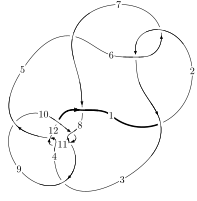
\includegraphics[width=112pt]{../../../GIT/diagram.site/Diagrams/png/1217_12a_0416.png}\\
\ \ \ A knot diagram\footnotemark}&
\allowdisplaybreaks
\textbf{Linearized knot diagam} \\
\cline{2-2}
 &
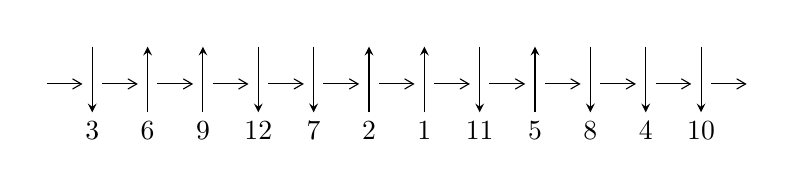
\begin{tikzpicture}[x=20pt, y=17pt]
	% nodes
	\node (C0) at (0, 0) {};
	\node (C1) at (1, 0) {};
	\node (C1U) at (1, +1) {};
	\node (C1D) at (1, -1) {3};

	\node (C2) at (2, 0) {};
	\node (C2U) at (2, +1) {};
	\node (C2D) at (2, -1) {6};

	\node (C3) at (3, 0) {};
	\node (C3U) at (3, +1) {};
	\node (C3D) at (3, -1) {9};

	\node (C4) at (4, 0) {};
	\node (C4U) at (4, +1) {};
	\node (C4D) at (4, -1) {12};

	\node (C5) at (5, 0) {};
	\node (C5U) at (5, +1) {};
	\node (C5D) at (5, -1) {7};

	\node (C6) at (6, 0) {};
	\node (C6U) at (6, +1) {};
	\node (C6D) at (6, -1) {2};

	\node (C7) at (7, 0) {};
	\node (C7U) at (7, +1) {};
	\node (C7D) at (7, -1) {1};

	\node (C8) at (8, 0) {};
	\node (C8U) at (8, +1) {};
	\node (C8D) at (8, -1) {11};

	\node (C9) at (9, 0) {};
	\node (C9U) at (9, +1) {};
	\node (C9D) at (9, -1) {5};

	\node (C10) at (10, 0) {};
	\node (C10U) at (10, +1) {};
	\node (C10D) at (10, -1) {8};

	\node (C11) at (11, 0) {};
	\node (C11U) at (11, +1) {};
	\node (C11D) at (11, -1) {4};

	\node (C12) at (12, 0) {};
	\node (C12U) at (12, +1) {};
	\node (C12D) at (12, -1) {10};
	\node (C13) at (13, 0) {};

	% arrows
	\draw[->,>={angle 60}]
	(C0) edge (C1) (C1) edge (C2) (C2) edge (C3) (C3) edge (C4) (C4) edge (C5) (C5) edge (C6) (C6) edge (C7) (C7) edge (C8) (C8) edge (C9) (C9) edge (C10) (C10) edge (C11) (C11) edge (C12) (C12) edge (C13) ;	\draw[->,>=stealth]
	(C1U) edge (C1D) (C2D) edge (C2U) (C3D) edge (C3U) (C4U) edge (C4D) (C5U) edge (C5D) (C6D) edge (C6U) (C7D) edge (C7U) (C8U) edge (C8D) (C9D) edge (C9U) (C10U) edge (C10D) (C11U) edge (C11D) (C12U) edge (C12D) ;
	\end{tikzpicture} \\
\hhline{~~} \\& 
\textbf{Solving Sequence} \\ \cline{2-2} 
 &
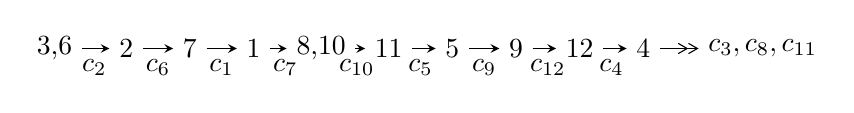
\begin{tikzpicture}[x=23pt, y=7pt]
	% node
	\node (A0) at (-1/8, 0) {3,6};
	\node (A1) at (1, 0) {2};
	\node (A2) at (2, 0) {7};
	\node (A3) at (3, 0) {1};
	\node (A4) at (65/16, 0) {8,10};
	\node (A5) at (41/8, 0) {11};
	\node (A6) at (49/8, 0) {5};
	\node (A7) at (57/8, 0) {9};
	\node (A8) at (65/8, 0) {12};
	\node (A9) at (73/8, 0) {4};
	\node (C1) at (1/2, -1) {$c_{2}$};
	\node (C2) at (3/2, -1) {$c_{6}$};
	\node (C3) at (5/2, -1) {$c_{1}$};
	\node (C4) at (7/2, -1) {$c_{7}$};
	\node (C5) at (37/8, -1) {$c_{10}$};
	\node (C6) at (45/8, -1) {$c_{5}$};
	\node (C7) at (53/8, -1) {$c_{9}$};
	\node (C8) at (61/8, -1) {$c_{12}$};
	\node (C9) at (69/8, -1) {$c_{4}$};
	\node (A10) at (11, 0) {$c_{3},c_{8},c_{11}$};

	% edge
	\draw[->,>=stealth]	
	(A0) edge (A1) (A1) edge (A2) (A2) edge (A3) (A3) edge (A4) (A4) edge (A5) (A5) edge (A6) (A6) edge (A7) (A7) edge (A8) (A8) edge (A9) ;
	\draw[->>,>={angle 60}]	
	(A9) edge (A10);
\end{tikzpicture} \\ 

\end{tabular} \\

\footnotetext{
The image of knot diagram is generated by the software ``\textbf{Draw programme}" developed by Andrew Bartholomew(\url{http://www.layer8.co.uk/maths/draw/index.htm\#Running-draw}), where we modified some parts for our purpose(\url{https://github.com/CATsTAILs/LinksPainter}).
}\phantom \\ \newline 
\centering \textbf{Ideals for irreducible components\footnotemark of $X_{\text{par}}$} 
 
\begin{align*}
I^u_{1}&=\langle 
6.41786\times10^{58} u^{106}+1.11346\times10^{59} u^{105}+\cdots+3.68055\times10^{58} b+3.69355\times10^{58},\\
\phantom{I^u_{1}}&\phantom{= \langle  }5.68621\times10^{58} u^{106}+8.00830\times10^{58} u^{105}+\cdots+3.68055\times10^{58} a+2.33644\times10^{58},\;u^{107}+2 u^{106}+\cdots+5 u^2+1\rangle \\
I^u_{2}&=\langle 
3 u^3-10 u^2+16 b+5 u-1,\;u^3+2 u^2+16 a-9 u+5,\;u^4- u^3+u^2+1\rangle \\
\\
\end{align*}
\raggedright * 2 irreducible components of $\dim_{\mathbb{C}}=0$, with total 111 representations.\\
\footnotetext{All coefficients of polynomials are rational numbers. But the coefficients are sometimes approximated in decimal forms when there is not enough margin.}
\newpage
\renewcommand{\arraystretch}{1}
\centering \section*{I. $I^u_{1}= \langle 6.42\times10^{58} u^{106}+1.11\times10^{59} u^{105}+\cdots+3.68\times10^{58} b+3.69\times10^{58},\;5.69\times10^{58} u^{106}+8.01\times10^{58} u^{105}+\cdots+3.68\times10^{58} a+2.34\times10^{58},\;u^{107}+2 u^{106}+\cdots+5 u^2+1 \rangle$}
\flushleft \textbf{(i) Arc colorings}\\
\begin{tabular}{m{7pt} m{180pt} m{7pt} m{180pt} }
\flushright $a_{3}=$&$\begin{pmatrix}1\\0\end{pmatrix}$ \\
\flushright $a_{6}=$&$\begin{pmatrix}0\\u\end{pmatrix}$ \\
\flushright $a_{2}=$&$\begin{pmatrix}1\\u^2\end{pmatrix}$ \\
\flushright $a_{7}=$&$\begin{pmatrix}u\\u^3+u\end{pmatrix}$ \\
\flushright $a_{1}=$&$\begin{pmatrix}u^2+1\\u^2\end{pmatrix}$ \\
\flushright $a_{8}=$&$\begin{pmatrix}u^7+2 u^5+2 u^3+2 u\\u^7+u^5+2 u^3+u\end{pmatrix}$ \\
\flushright $a_{10}=$&$\begin{pmatrix}-1.54494 u^{106}-2.17584 u^{105}+\cdots+4.67915 u-0.634808\\-1.74372 u^{106}-3.02525 u^{105}+\cdots-0.345092 u-1.00353\end{pmatrix}$ \\
\flushright $a_{11}=$&$\begin{pmatrix}-1.61452 u^{106}-2.12033 u^{105}+\cdots+2.40127 u-0.833938\\-1.79319 u^{106}-3.10408 u^{105}+\cdots-1.51075 u-1.20808\end{pmatrix}$ \\
\flushright $a_{5}=$&$\begin{pmatrix}u^3\\u^5+u^3+u\end{pmatrix}$ \\
\flushright $a_{9}=$&$\begin{pmatrix}-1.30918 u^{106}-1.99248 u^{105}+\cdots+4.75193 u-0.619919\\-1.49000 u^{106}-2.55809 u^{105}+\cdots-0.284829 u-0.785527\end{pmatrix}$ \\
\flushright $a_{12}=$&$\begin{pmatrix}1.91247 u^{106}+1.68905 u^{105}+\cdots+0.287353 u-2.38447\\1.66556 u^{106}+3.26726 u^{105}+\cdots+3.40325 u+0.816457\end{pmatrix}$ \\
\flushright $a_{4}=$&$\begin{pmatrix}-0.193027 u^{106}+0.449266 u^{105}+\cdots-2.00140 u+0.00824800\\0.232615 u^{106}+0.0280210 u^{105}+\cdots+4.32238 u-1.20722\end{pmatrix}$\\&\end{tabular}
\flushleft \textbf{(ii) Obstruction class $= -1$}\\~\\
\flushleft \textbf{(iii) Cusp Shapes $= 0.124020 u^{106}-0.719172 u^{105}+\cdots-1.22907 u-7.39183$}\\~\\
\newpage\renewcommand{\arraystretch}{1}
\flushleft \textbf{(iv) u-Polynomials at the component}\newline \\
\begin{tabular}{m{50pt}|m{274pt}}
Crossings & \hspace{64pt}u-Polynomials at each crossing \\
\hline $$\begin{aligned}c_{1},c_{5}\end{aligned}$$&$\begin{aligned}
&u^{107}+36 u^{106}+\cdots-10 u-1
\end{aligned}$\\
\hline $$\begin{aligned}c_{2},c_{6}\end{aligned}$$&$\begin{aligned}
&u^{107}-2 u^{106}+\cdots-5 u^2-1
\end{aligned}$\\
\hline $$\begin{aligned}c_{3}\end{aligned}$$&$\begin{aligned}
&16(16 u^{107}-75 u^{106}+\cdots-2.85939\times10^{8} u-5.57740\times10^{7})
\end{aligned}$\\
\hline $$\begin{aligned}c_{4},c_{11}\end{aligned}$$&$\begin{aligned}
&u^{107}+2 u^{106}+\cdots+4 u+1
\end{aligned}$\\
\hline $$\begin{aligned}c_{7}\end{aligned}$$&$\begin{aligned}
&u^{107}+10 u^{106}+\cdots-55360 u-60751
\end{aligned}$\\
\hline $$\begin{aligned}c_{8},c_{10}\end{aligned}$$&$\begin{aligned}
&u^{107}-5 u^{106}+\cdots+3671 u+256
\end{aligned}$\\
\hline $$\begin{aligned}c_{9}\end{aligned}$$&$\begin{aligned}
&u^{107}-3 u^{106}+\cdots-14208 u-4096
\end{aligned}$\\
\hline $$\begin{aligned}c_{12}\end{aligned}$$&$\begin{aligned}
&16(16 u^{107}+83 u^{106}+\cdots+1.25403\times10^{8} u-9972353)
\end{aligned}$\\
\hline
\end{tabular}\\~\\
\newpage\renewcommand{\arraystretch}{1}
\flushleft \textbf{(v) Riley Polynomials at the component}\newline \\
\begin{tabular}{m{50pt}|m{274pt}}
Crossings & \hspace{64pt}Riley Polynomials at each crossing \\
\hline $$\begin{aligned}c_{1},c_{5}\end{aligned}$$&$\begin{aligned}
&y^{107}+72 y^{106}+\cdots-22 y-1
\end{aligned}$\\
\hline $$\begin{aligned}c_{2},c_{6}\end{aligned}$$&$\begin{aligned}
&y^{107}+36 y^{106}+\cdots-10 y-1
\end{aligned}$\\
\hline $$\begin{aligned}c_{3}\end{aligned}$$&$\begin{aligned}
&256(256 y^{107}+25319 y^{106}+\cdots-7.95186\times10^{16} y-3.11074\times10^{15})
\end{aligned}$\\
\hline $$\begin{aligned}c_{4},c_{11}\end{aligned}$$&$\begin{aligned}
&y^{107}-72 y^{106}+\cdots-10 y-1
\end{aligned}$\\
\hline $$\begin{aligned}c_{7}\end{aligned}$$&$\begin{aligned}
&y^{107}+36 y^{106}+\cdots-86065371038 y-3690684001
\end{aligned}$\\
\hline $$\begin{aligned}c_{8},c_{10}\end{aligned}$$&$\begin{aligned}
&y^{107}-85 y^{106}+\cdots+5667729 y-65536
\end{aligned}$\\
\hline $$\begin{aligned}c_{9}\end{aligned}$$&$\begin{aligned}
&y^{107}+27 y^{106}+\cdots-1042857984 y-16777216
\end{aligned}$\\
\hline $$\begin{aligned}c_{12}\end{aligned}$$&$\begin{aligned}
&256\\
&\cdot(256 y^{107}-3401 y^{106}+\cdots+3072980132794765 y-99447824356609)
\end{aligned}$\\
\hline
\end{tabular}\\~\\
\newpage\flushleft \textbf{(vi) Complex Volumes and Cusp Shapes}
$$\begin{array}{c|c|c}  
\text{Solutions to }I^u_{1}& \I (\text{vol} + \sqrt{-1}CS) & \text{Cusp shape}\\
 \hline 
\begin{aligned}
u &= \phantom{-}0.572555 + 0.816228 I \\
a &= \phantom{-}2.52809 + 0.77404 I \\
b &= \phantom{-}0.51685 + 1.60831 I\end{aligned}
 & -2.67149 + 4.54950 I & \phantom{-0.000000 } 0 \\ \hline\begin{aligned}
u &= \phantom{-}0.572555 - 0.816228 I \\
a &= \phantom{-}2.52809 - 0.77404 I \\
b &= \phantom{-}0.51685 - 1.60831 I\end{aligned}
 & -2.67149 - 4.54950 I & \phantom{-0.000000 } 0 \\ \hline\begin{aligned}
u &= -0.739110 + 0.684442 I \\
a &= \phantom{-}1.64740 + 0.61961 I \\
b &= \phantom{-}1.54687 + 0.42061 I\end{aligned}
 & -0.333003 + 0.042241 I & \phantom{-0.000000 } 0 \\ \hline\begin{aligned}
u &= -0.739110 - 0.684442 I \\
a &= \phantom{-}1.64740 - 0.61961 I \\
b &= \phantom{-}1.54687 - 0.42061 I\end{aligned}
 & -0.333003 - 0.042241 I & \phantom{-0.000000 } 0 \\ \hline\begin{aligned}
u &= \phantom{-}0.693461 + 0.733009 I \\
a &= \phantom{-}0.96918 + 4.82361 I \\
b &= \phantom{-}0.47980 + 4.66509 I\end{aligned}
 & -1.47357 - 0.02935 I & \phantom{-0.000000 } 0 \\ \hline\begin{aligned}
u &= \phantom{-}0.693461 - 0.733009 I \\
a &= \phantom{-}0.96918 - 4.82361 I \\
b &= \phantom{-}0.47980 - 4.66509 I\end{aligned}
 & -1.47357 + 0.02935 I & \phantom{-0.000000 } 0 \\ \hline\begin{aligned}
u &= -0.647407 + 0.776662 I \\
a &= -1.38461 + 0.99050 I \\
b &= -0.48414 + 1.42730 I\end{aligned}
 & \phantom{-}0.84772 - 2.11192 I & \phantom{-0.000000 } 0 \\ \hline\begin{aligned}
u &= -0.647407 - 0.776662 I \\
a &= -1.38461 - 0.99050 I \\
b &= -0.48414 - 1.42730 I\end{aligned}
 & \phantom{-}0.84772 + 2.11192 I & \phantom{-0.000000 } 0 \\ \hline\begin{aligned}
u &= \phantom{-}0.046668 + 1.012190 I \\
a &= \phantom{-}1.11018 + 1.35436 I \\
b &= -1.68594 - 1.42232 I\end{aligned}
 & -5.79533 - 0.00929 I & \phantom{-0.000000 } 0 \\ \hline\begin{aligned}
u &= \phantom{-}0.046668 - 1.012190 I \\
a &= \phantom{-}1.11018 - 1.35436 I \\
b &= -1.68594 + 1.42232 I\end{aligned}
 & -5.79533 + 0.00929 I & \phantom{-0.000000 } 0\\
 \hline 
 \end{array}$$\newpage$$\begin{array}{c|c|c}  
\text{Solutions to }I^u_{1}& \I (\text{vol} + \sqrt{-1}CS) & \text{Cusp shape}\\
 \hline 
\begin{aligned}
u &= -0.779058 + 0.650419 I \\
a &= \phantom{-}2.55013 - 1.30493 I \\
b &= \phantom{-}1.56781 - 1.66329 I\end{aligned}
 & -0.45641 + 6.27660 I & \phantom{-0.000000 } 0 \\ \hline\begin{aligned}
u &= -0.779058 - 0.650419 I \\
a &= \phantom{-}2.55013 + 1.30493 I \\
b &= \phantom{-}1.56781 + 1.66329 I\end{aligned}
 & -0.45641 - 6.27660 I & \phantom{-0.000000 } 0 \\ \hline\begin{aligned}
u &= -0.718616 + 0.656188 I \\
a &= \phantom{-}1.50113 - 0.25187 I \\
b &= \phantom{-}1.54019 - 1.12578 I\end{aligned}
 & -0.67697 + 1.53545 I & \phantom{-0.000000 } 0 \\ \hline\begin{aligned}
u &= -0.718616 - 0.656188 I \\
a &= \phantom{-}1.50113 + 0.25187 I \\
b &= \phantom{-}1.54019 + 1.12578 I\end{aligned}
 & -0.67697 - 1.53545 I & \phantom{-0.000000 } 0 \\ \hline\begin{aligned}
u &= \phantom{-}0.777566 + 0.672502 I \\
a &= -1.70061 - 0.94033 I \\
b &= -1.06308 - 1.09985 I\end{aligned}
 & \phantom{-}3.07553 - 2.64129 I & \phantom{-0.000000 } 0 \\ \hline\begin{aligned}
u &= \phantom{-}0.777566 - 0.672502 I \\
a &= -1.70061 + 0.94033 I \\
b &= -1.06308 + 1.09985 I\end{aligned}
 & \phantom{-}3.07553 + 2.64129 I & \phantom{-0.000000 } 0 \\ \hline\begin{aligned}
u &= -0.078882 + 1.030440 I \\
a &= -0.621536 + 0.191873 I \\
b &= \phantom{-}1.48564 + 0.21337 I\end{aligned}
 & -2.81526 - 2.54077 I & \phantom{-0.000000 } 0 \\ \hline\begin{aligned}
u &= -0.078882 - 1.030440 I \\
a &= -0.621536 - 0.191873 I \\
b &= \phantom{-}1.48564 - 0.21337 I\end{aligned}
 & -2.81526 + 2.54077 I & \phantom{-0.000000 } 0 \\ \hline\begin{aligned}
u &= \phantom{-}0.018006 + 1.038180 I \\
a &= \phantom{-}1.04825 - 1.03206 I \\
b &= -1.51635 + 0.37279 I\end{aligned}
 & -5.96646 + 1.12046 I & \phantom{-0.000000 } 0 \\ \hline\begin{aligned}
u &= \phantom{-}0.018006 - 1.038180 I \\
a &= \phantom{-}1.04825 + 1.03206 I \\
b &= -1.51635 - 0.37279 I\end{aligned}
 & -5.96646 - 1.12046 I & \phantom{-0.000000 } 0\\
 \hline 
 \end{array}$$\newpage$$\begin{array}{c|c|c}  
\text{Solutions to }I^u_{1}& \I (\text{vol} + \sqrt{-1}CS) & \text{Cusp shape}\\
 \hline 
\begin{aligned}
u &= \phantom{-}0.727533 + 0.620282 I \\
a &= -2.21540 + 1.31033 I \\
b &= -1.97976 - 0.19879 I\end{aligned}
 & -5.08482 - 3.05325 I & \phantom{-0.000000 } 0 \\ \hline\begin{aligned}
u &= \phantom{-}0.727533 - 0.620282 I \\
a &= -2.21540 - 1.31033 I \\
b &= -1.97976 + 0.19879 I\end{aligned}
 & -5.08482 + 3.05325 I & \phantom{-0.000000 } 0 \\ \hline\begin{aligned}
u &= \phantom{-}0.837675 + 0.627096 I \\
a &= \phantom{-}1.61326 + 0.70242 I \\
b &= \phantom{-}1.42239 + 1.01685 I\end{aligned}
 & -0.72153 - 6.99583 I & \phantom{-0.000000 } 0 \\ \hline\begin{aligned}
u &= \phantom{-}0.837675 - 0.627096 I \\
a &= \phantom{-}1.61326 - 0.70242 I \\
b &= \phantom{-}1.42239 - 1.01685 I\end{aligned}
 & -0.72153 + 6.99583 I & \phantom{-0.000000 } 0 \\ \hline\begin{aligned}
u &= -0.833095 + 0.636825 I \\
a &= -2.29893 + 0.83993 I \\
b &= -1.98652 + 1.23353 I\end{aligned}
 & -5.55745 + 12.65750 I & \phantom{-0.000000 } 0 \\ \hline\begin{aligned}
u &= -0.833095 - 0.636825 I \\
a &= -2.29893 - 0.83993 I \\
b &= -1.98652 - 1.23353 I\end{aligned}
 & -5.55745 - 12.65750 I & \phantom{-0.000000 } 0 \\ \hline\begin{aligned}
u &= \phantom{-}0.663407 + 0.676201 I \\
a &= \phantom{-}1.72189 + 0.62515 I \\
b &= \phantom{-}0.962894 - 0.088589 I\end{aligned}
 & -1.161400 + 0.572745 I & \phantom{-0.000000 } 0 \\ \hline\begin{aligned}
u &= \phantom{-}0.663407 - 0.676201 I \\
a &= \phantom{-}1.72189 - 0.62515 I \\
b &= \phantom{-}0.962894 + 0.088589 I\end{aligned}
 & -1.161400 - 0.572745 I & \phantom{-0.000000 } 0 \\ \hline\begin{aligned}
u &= \phantom{-}0.072508 + 1.059040 I \\
a &= \phantom{-}0.718322 - 0.057892 I \\
b &= -2.23899 + 0.56383 I\end{aligned}
 & -6.38996 + 5.89641 I & \phantom{-0.000000 } 0 \\ \hline\begin{aligned}
u &= \phantom{-}0.072508 - 1.059040 I \\
a &= \phantom{-}0.718322 + 0.057892 I \\
b &= -2.23899 - 0.56383 I\end{aligned}
 & -6.38996 - 5.89641 I & \phantom{-0.000000 } 0\\
 \hline 
 \end{array}$$\newpage$$\begin{array}{c|c|c}  
\text{Solutions to }I^u_{1}& \I (\text{vol} + \sqrt{-1}CS) & \text{Cusp shape}\\
 \hline 
\begin{aligned}
u &= -0.021482 + 1.065870 I \\
a &= -0.498349 - 0.295555 I \\
b &= \phantom{-}1.57487 - 1.20386 I\end{aligned}
 & -10.53900 - 2.34670 I & \phantom{-0.000000 } 0 \\ \hline\begin{aligned}
u &= -0.021482 - 1.065870 I \\
a &= -0.498349 + 0.295555 I \\
b &= \phantom{-}1.57487 + 1.20386 I\end{aligned}
 & -10.53900 + 2.34670 I & \phantom{-0.000000 } 0 \\ \hline\begin{aligned}
u &= -0.861913 + 0.640246 I \\
a &= -1.127330 - 0.215348 I \\
b &= -1.160100 + 0.147222 I\end{aligned}
 & -4.62472 + 0.42113 I & \phantom{-0.000000 } 0 \\ \hline\begin{aligned}
u &= -0.861913 - 0.640246 I \\
a &= -1.127330 + 0.215348 I \\
b &= -1.160100 - 0.147222 I\end{aligned}
 & -4.62472 - 0.42113 I & \phantom{-0.000000 } 0 \\ \hline\begin{aligned}
u &= -0.733935 + 0.841377 I \\
a &= -0.207227 - 0.928291 I \\
b &= -0.919580 + 0.275183 I\end{aligned}
 & \phantom{-}2.46950 - 5.13290 I & \phantom{-0.000000 } 0 \\ \hline\begin{aligned}
u &= -0.733935 - 0.841377 I \\
a &= -0.207227 + 0.928291 I \\
b &= -0.919580 - 0.275183 I\end{aligned}
 & \phantom{-}2.46950 + 5.13290 I & \phantom{-0.000000 } 0 \\ \hline\begin{aligned}
u &= \phantom{-}0.111769 + 1.113810 I \\
a &= -0.968189 - 0.007849 I \\
b &= \phantom{-}2.09870 - 0.48022 I\end{aligned}
 & -12.1009 + 12.0094 I & \phantom{-0.000000 } 0 \\ \hline\begin{aligned}
u &= \phantom{-}0.111769 - 1.113810 I \\
a &= -0.968189 + 0.007849 I \\
b &= \phantom{-}2.09870 + 0.48022 I\end{aligned}
 & -12.1009 - 12.0094 I & \phantom{-0.000000 } 0 \\ \hline\begin{aligned}
u &= \phantom{-}0.765238 + 0.818174 I \\
a &= -0.212152 - 0.487781 I \\
b &= \phantom{-}0.491573 + 0.001552 I\end{aligned}
 & \phantom{-}5.25937 + 0.90397 I & \phantom{-0.000000 } 0 \\ \hline\begin{aligned}
u &= \phantom{-}0.765238 - 0.818174 I \\
a &= -0.212152 + 0.487781 I \\
b &= \phantom{-}0.491573 - 0.001552 I\end{aligned}
 & \phantom{-}5.25937 - 0.90397 I & \phantom{-0.000000 } 0\\
 \hline 
 \end{array}$$\newpage$$\begin{array}{c|c|c}  
\text{Solutions to }I^u_{1}& \I (\text{vol} + \sqrt{-1}CS) & \text{Cusp shape}\\
 \hline 
\begin{aligned}
u &= -0.634185 + 0.597497 I \\
a &= -1.20096 + 2.39832 I \\
b &= \phantom{-}0.044086 + 0.934957 I\end{aligned}
 & -5.60148 - 1.35298 I & \phantom{-0.000000 } 0 \\ \hline\begin{aligned}
u &= -0.634185 - 0.597497 I \\
a &= -1.20096 - 2.39832 I \\
b &= \phantom{-}0.044086 - 0.934957 I\end{aligned}
 & -5.60148 + 1.35298 I & \phantom{-0.000000 } 0 \\ \hline\begin{aligned}
u &= -0.109524 + 1.125450 I \\
a &= \phantom{-}0.705092 + 0.077937 I \\
b &= -1.49776 - 0.36174 I\end{aligned}
 & -7.29613 - 6.22971 I & \phantom{-0.000000 } 0 \\ \hline\begin{aligned}
u &= -0.109524 - 1.125450 I \\
a &= \phantom{-}0.705092 - 0.077937 I \\
b &= -1.49776 + 0.36174 I\end{aligned}
 & -7.29613 + 6.22971 I & \phantom{-0.000000 } 0 \\ \hline\begin{aligned}
u &= \phantom{-}0.132569 + 1.127410 I \\
a &= -0.452270 - 0.144598 I \\
b &= \phantom{-}1.151400 + 0.385658 I\end{aligned}
 & -11.45990 - 0.25981 I & \phantom{-0.000000 } 0 \\ \hline\begin{aligned}
u &= \phantom{-}0.132569 - 1.127410 I \\
a &= -0.452270 + 0.144598 I \\
b &= \phantom{-}1.151400 - 0.385658 I\end{aligned}
 & -11.45990 + 0.25981 I & \phantom{-0.000000 } 0 \\ \hline\begin{aligned}
u &= -0.721484 + 0.881806 I \\
a &= \phantom{-}0.287036 + 0.095689 I \\
b &= \phantom{-}1.006650 - 0.068646 I\end{aligned}
 & \phantom{-}2.34405 - 0.40468 I & \phantom{-0.000000 } 0 \\ \hline\begin{aligned}
u &= -0.721484 - 0.881806 I \\
a &= \phantom{-}0.287036 - 0.095689 I \\
b &= \phantom{-}1.006650 + 0.068646 I\end{aligned}
 & \phantom{-}2.34405 + 0.40468 I & \phantom{-0.000000 } 0 \\ \hline\begin{aligned}
u &= -0.636751 + 0.946553 I \\
a &= -0.38190 + 1.89505 I \\
b &= \phantom{-}1.13597 + 1.16685 I\end{aligned}
 & \phantom{-}0.30477 - 2.89231 I & \phantom{-0.000000 } 0 \\ \hline\begin{aligned}
u &= -0.636751 - 0.946553 I \\
a &= -0.38190 - 1.89505 I \\
b &= \phantom{-}1.13597 - 1.16685 I\end{aligned}
 & \phantom{-}0.30477 + 2.89231 I & \phantom{-0.000000 } 0\\
 \hline 
 \end{array}$$\newpage$$\begin{array}{c|c|c}  
\text{Solutions to }I^u_{1}& \I (\text{vol} + \sqrt{-1}CS) & \text{Cusp shape}\\
 \hline 
\begin{aligned}
u &= \phantom{-}0.605466 + 0.969047 I \\
a &= -0.47718 + 2.60038 I \\
b &= -1.75712 + 1.09425 I\end{aligned}
 & -3.29947 + 0.02397 I & \phantom{-0.000000 } 0 \\ \hline\begin{aligned}
u &= \phantom{-}0.605466 - 0.969047 I \\
a &= -0.47718 - 2.60038 I \\
b &= -1.75712 - 1.09425 I\end{aligned}
 & -3.29947 - 0.02397 I & \phantom{-0.000000 } 0 \\ \hline\begin{aligned}
u &= \phantom{-}0.501653 + 1.045680 I \\
a &= -0.76284 - 1.21835 I \\
b &= \phantom{-}0.416918 - 0.654919 I\end{aligned}
 & -9.20052 + 7.31020 I & \phantom{-0.000000 } 0 \\ \hline\begin{aligned}
u &= \phantom{-}0.501653 - 1.045680 I \\
a &= -0.76284 + 1.21835 I \\
b &= \phantom{-}0.416918 + 0.654919 I\end{aligned}
 & -9.20052 - 7.31020 I & \phantom{-0.000000 } 0 \\ \hline\begin{aligned}
u &= \phantom{-}0.531187 + 1.038580 I \\
a &= \phantom{-}0.38097 - 2.08084 I \\
b &= \phantom{-}1.352130 - 0.228748 I\end{aligned}
 & -9.54319 - 5.13852 I & \phantom{-0.000000 } 0 \\ \hline\begin{aligned}
u &= \phantom{-}0.531187 - 1.038580 I \\
a &= \phantom{-}0.38097 + 2.08084 I \\
b &= \phantom{-}1.352130 + 0.228748 I\end{aligned}
 & -9.54319 + 5.13852 I & \phantom{-0.000000 } 0 \\ \hline\begin{aligned}
u &= -0.245463 + 0.792676 I \\
a &= \phantom{-}0.199411 + 0.599935 I \\
b &= \phantom{-}0.271663 + 0.310043 I\end{aligned}
 & -0.56851 - 1.64515 I & \phantom{-0.000000 -}0. + 5.38816 I \\ \hline\begin{aligned}
u &= -0.245463 - 0.792676 I \\
a &= \phantom{-}0.199411 - 0.599935 I \\
b &= \phantom{-}0.271663 - 0.310043 I\end{aligned}
 & -0.56851 + 1.64515 I & \phantom{-0.000000 } 0. - 5.38816 I \\ \hline\begin{aligned}
u &= \phantom{-}0.665165 + 0.963024 I \\
a &= \phantom{-}3.68761 + 3.95714 I \\
b &= -1.50055 + 3.53640 I\end{aligned}
 & -2.17929 + 5.27880 I & \phantom{-0.000000 } 0 \\ \hline\begin{aligned}
u &= \phantom{-}0.665165 - 0.963024 I \\
a &= \phantom{-}3.68761 - 3.95714 I \\
b &= -1.50055 - 3.53640 I\end{aligned}
 & -2.17929 - 5.27880 I & \phantom{-0.000000 } 0\\
 \hline 
 \end{array}$$\newpage$$\begin{array}{c|c|c}  
\text{Solutions to }I^u_{1}& \I (\text{vol} + \sqrt{-1}CS) & \text{Cusp shape}\\
 \hline 
\begin{aligned}
u &= \phantom{-}0.745883 + 0.914563 I \\
a &= -0.0171571 - 0.0566864 I \\
b &= -0.494211 - 0.276217 I\end{aligned}
 & \phantom{-}4.96743 + 4.80385 I & \phantom{-0.000000 } 0 \\ \hline\begin{aligned}
u &= \phantom{-}0.745883 - 0.914563 I \\
a &= -0.0171571 + 0.0566864 I \\
b &= -0.494211 + 0.276217 I\end{aligned}
 & \phantom{-}4.96743 - 4.80385 I & \phantom{-0.000000 } 0 \\ \hline\begin{aligned}
u &= -0.811697 + 0.857361 I \\
a &= \phantom{-}0.450118 - 0.099056 I \\
b &= -0.312448 - 0.472158 I\end{aligned}
 & -0.73668 + 3.73977 I & \phantom{-0.000000 } 0 \\ \hline\begin{aligned}
u &= -0.811697 - 0.857361 I \\
a &= \phantom{-}0.450118 + 0.099056 I \\
b &= -0.312448 + 0.472158 I\end{aligned}
 & -0.73668 - 3.73977 I & \phantom{-0.000000 } 0 \\ \hline\begin{aligned}
u &= -0.529166 + 1.057900 I \\
a &= -0.137429 - 1.371400 I \\
b &= -0.821551 - 0.155925 I\end{aligned}
 & -4.70260 - 0.83335 I & \phantom{-0.000000 } 0 \\ \hline\begin{aligned}
u &= -0.529166 - 1.057900 I \\
a &= -0.137429 + 1.371400 I \\
b &= -0.821551 + 0.155925 I\end{aligned}
 & -4.70260 + 0.83335 I & \phantom{-0.000000 } 0 \\ \hline\begin{aligned}
u &= \phantom{-}0.656100 + 0.987672 I \\
a &= -1.02169 + 2.13604 I \\
b &= -1.127310 + 0.026416 I\end{aligned}
 & -2.10121 + 4.59471 I & \phantom{-0.000000 } 0 \\ \hline\begin{aligned}
u &= \phantom{-}0.656100 - 0.987672 I \\
a &= -1.02169 - 2.13604 I \\
b &= -1.127310 - 0.026416 I\end{aligned}
 & -2.10121 - 4.59471 I & \phantom{-0.000000 } 0 \\ \hline\begin{aligned}
u &= -0.641946 + 1.002990 I \\
a &= -1.20790 + 2.08709 I \\
b &= \phantom{-}0.15928 + 1.79219 I\end{aligned}
 & -6.75012 - 3.71244 I & \phantom{-0.000000 } 0 \\ \hline\begin{aligned}
u &= -0.641946 - 1.002990 I \\
a &= -1.20790 - 2.08709 I \\
b &= \phantom{-}0.15928 - 1.79219 I\end{aligned}
 & -6.75012 + 3.71244 I & \phantom{-0.000000 } 0\\
 \hline 
 \end{array}$$\newpage$$\begin{array}{c|c|c}  
\text{Solutions to }I^u_{1}& \I (\text{vol} + \sqrt{-1}CS) & \text{Cusp shape}\\
 \hline 
\begin{aligned}
u &= -0.749094 + 0.305561 I \\
a &= \phantom{-}1.051380 - 0.015805 I \\
b &= \phantom{-}0.884161 + 0.341399 I\end{aligned}
 & -2.47323 - 3.82700 I & -4.04906 + 6.12784 I \\ \hline\begin{aligned}
u &= -0.749094 - 0.305561 I \\
a &= \phantom{-}1.051380 + 0.015805 I \\
b &= \phantom{-}0.884161 - 0.341399 I\end{aligned}
 & -2.47323 + 3.82700 I & -4.04906 - 6.12784 I \\ \hline\begin{aligned}
u &= -0.794258 + 0.900063 I \\
a &= \phantom{-}0.0218861 + 0.0446674 I \\
b &= \phantom{-}0.161813 - 0.644801 I\end{aligned}
 & -0.87138 - 9.73384 I & \phantom{-0.000000 } 0 \\ \hline\begin{aligned}
u &= -0.794258 - 0.900063 I \\
a &= \phantom{-}0.0218861 - 0.0446674 I \\
b &= \phantom{-}0.161813 + 0.644801 I\end{aligned}
 & -0.87138 + 9.73384 I & \phantom{-0.000000 } 0 \\ \hline\begin{aligned}
u &= -0.672273 + 1.000660 I \\
a &= \phantom{-}0.36256 - 2.06486 I \\
b &= -1.85620 - 0.99758 I\end{aligned}
 & -1.70112 - 6.88767 I & \phantom{-0.000000 } 0 \\ \hline\begin{aligned}
u &= -0.672273 - 1.000660 I \\
a &= \phantom{-}0.36256 + 2.06486 I \\
b &= -1.85620 + 0.99758 I\end{aligned}
 & -1.70112 + 6.88767 I & \phantom{-0.000000 } 0 \\ \hline\begin{aligned}
u &= -0.688074 + 0.993783 I \\
a &= -1.68115 - 1.97202 I \\
b &= -1.87014 + 0.44496 I\end{aligned}
 & -1.26073 - 5.50150 I & \phantom{-0.000000 } 0 \\ \hline\begin{aligned}
u &= -0.688074 - 0.993783 I \\
a &= -1.68115 + 1.97202 I \\
b &= -1.87014 - 0.44496 I\end{aligned}
 & -1.26073 + 5.50150 I & \phantom{-0.000000 } 0 \\ \hline\begin{aligned}
u &= \phantom{-}0.667865 + 1.014470 I \\
a &= \phantom{-}1.59065 - 1.79707 I \\
b &= \phantom{-}2.56053 + 0.11805 I\end{aligned}
 & -6.24275 + 8.40853 I & \phantom{-0.000000 } 0 \\ \hline\begin{aligned}
u &= \phantom{-}0.667865 - 1.014470 I \\
a &= \phantom{-}1.59065 + 1.79707 I \\
b &= \phantom{-}2.56053 - 0.11805 I\end{aligned}
 & -6.24275 - 8.40853 I & \phantom{-0.000000 } 0\\
 \hline 
 \end{array}$$\newpage$$\begin{array}{c|c|c}  
\text{Solutions to }I^u_{1}& \I (\text{vol} + \sqrt{-1}CS) & \text{Cusp shape}\\
 \hline 
\begin{aligned}
u &= \phantom{-}0.746220 + 0.243908 I \\
a &= -0.548011 - 0.781846 I \\
b &= -0.682427 - 0.253394 I\end{aligned}
 & -6.82390 - 2.87754 I & -7.55606 + 2.65618 I \\ \hline\begin{aligned}
u &= \phantom{-}0.746220 - 0.243908 I \\
a &= -0.548011 + 0.781846 I \\
b &= -0.682427 + 0.253394 I\end{aligned}
 & -6.82390 + 2.87754 I & -7.55606 - 2.65618 I \\ \hline\begin{aligned}
u &= \phantom{-}0.717094 + 0.295055 I \\
a &= -1.73531 - 0.02894 I \\
b &= -1.35567 + 0.43051 I\end{aligned}
 & -7.41312 + 9.67363 I & -4.73264 - 6.38997 I \\ \hline\begin{aligned}
u &= \phantom{-}0.717094 - 0.295055 I \\
a &= -1.73531 + 0.02894 I \\
b &= -1.35567 - 0.43051 I\end{aligned}
 & -7.41312 - 9.67363 I & -4.73264 + 6.38997 I \\ \hline\begin{aligned}
u &= \phantom{-}0.699336 + 1.008630 I \\
a &= -0.14409 - 2.25681 I \\
b &= \phantom{-}1.39931 - 1.21172 I\end{aligned}
 & \phantom{-}2.06203 + 8.23607 I & \phantom{-0.000000 } 0 \\ \hline\begin{aligned}
u &= \phantom{-}0.699336 - 1.008630 I \\
a &= -0.14409 + 2.25681 I \\
b &= \phantom{-}1.39931 + 1.21172 I\end{aligned}
 & \phantom{-}2.06203 - 8.23607 I & \phantom{-0.000000 } 0 \\ \hline\begin{aligned}
u &= -0.693869 + 1.018100 I \\
a &= \phantom{-}0.30703 - 3.14528 I \\
b &= -2.01636 - 1.87103 I\end{aligned}
 & -1.55940 - 11.85470 I & \phantom{-0.000000 } 0 \\ \hline\begin{aligned}
u &= -0.693869 - 1.018100 I \\
a &= \phantom{-}0.30703 + 3.14528 I \\
b &= -2.01636 + 1.87103 I\end{aligned}
 & -1.55940 + 11.85470 I & \phantom{-0.000000 } 0 \\ \hline\begin{aligned}
u &= \phantom{-}0.865077 + 0.912693 I \\
a &= -0.147695 - 0.056476 I \\
b &= \phantom{-}0.017267 - 0.336869 I\end{aligned}
 & \phantom{-}5.02105 + 3.20233 I & \phantom{-0.000000 } 0 \\ \hline\begin{aligned}
u &= \phantom{-}0.865077 - 0.912693 I \\
a &= -0.147695 + 0.056476 I \\
b &= \phantom{-}0.017267 + 0.336869 I\end{aligned}
 & \phantom{-}5.02105 - 3.20233 I & \phantom{-0.000000 } 0\\
 \hline 
 \end{array}$$\newpage$$\begin{array}{c|c|c}  
\text{Solutions to }I^u_{1}& \I (\text{vol} + \sqrt{-1}CS) & \text{Cusp shape}\\
 \hline 
\begin{aligned}
u &= -0.710551 + 1.042030 I \\
a &= \phantom{-}0.03854 + 2.97997 I \\
b &= \phantom{-}2.27288 + 1.28431 I\end{aligned}
 & -6.7863 - 18.4344 I & \phantom{-0.000000 } 0 \\ \hline\begin{aligned}
u &= -0.710551 - 1.042030 I \\
a &= \phantom{-}0.03854 - 2.97997 I \\
b &= \phantom{-}2.27288 - 1.28431 I\end{aligned}
 & -6.7863 + 18.4344 I & \phantom{-0.000000 } 0 \\ \hline\begin{aligned}
u &= \phantom{-}0.708638 + 1.046960 I \\
a &= \phantom{-}0.13873 + 2.21107 I \\
b &= -1.68135 + 1.06324 I\end{aligned}
 & -1.99428 + 12.77590 I & \phantom{-0.000000 } 0 \\ \hline\begin{aligned}
u &= \phantom{-}0.708638 - 1.046960 I \\
a &= \phantom{-}0.13873 - 2.21107 I \\
b &= -1.68135 - 1.06324 I\end{aligned}
 & -1.99428 - 12.77590 I & \phantom{-0.000000 } 0 \\ \hline\begin{aligned}
u &= -0.720384 + 1.052700 I \\
a &= \phantom{-}0.540882 + 1.306510 I \\
b &= \phantom{-}1.362950 + 0.189864 I\end{aligned}
 & -5.89103 - 6.31209 I & \phantom{-0.000000 } 0 \\ \hline\begin{aligned}
u &= -0.720384 - 1.052700 I \\
a &= \phantom{-}0.540882 - 1.306510 I \\
b &= \phantom{-}1.362950 - 0.189864 I\end{aligned}
 & -5.89103 + 6.31209 I & \phantom{-0.000000 } 0 \\ \hline\begin{aligned}
u &= -0.219769 + 0.626637 I \\
a &= -1.28173 + 2.73269 I \\
b &= \phantom{-}0.397565 - 0.307830 I\end{aligned}
 & -5.57963 - 1.60313 I & -10.66319 + 3.91153 I \\ \hline\begin{aligned}
u &= -0.219769 - 0.626637 I \\
a &= -1.28173 - 2.73269 I \\
b &= \phantom{-}0.397565 + 0.307830 I\end{aligned}
 & -5.57963 + 1.60313 I & -10.66319 - 3.91153 I \\ \hline\begin{aligned}
u &= \phantom{-}0.530510 + 0.326469 I \\
a &= \phantom{-}2.34754 + 0.32620 I \\
b &= \phantom{-}0.902410 - 0.116640 I\end{aligned}
 & -2.07804 + 4.29773 I & -3.00401 - 7.13446 I \\ \hline\begin{aligned}
u &= \phantom{-}0.530510 - 0.326469 I \\
a &= \phantom{-}2.34754 - 0.32620 I \\
b &= \phantom{-}0.902410 + 0.116640 I\end{aligned}
 & -2.07804 - 4.29773 I & -3.00401 + 7.13446 I\\
 \hline 
 \end{array}$$\newpage$$\begin{array}{c|c|c}  
\text{Solutions to }I^u_{1}& \I (\text{vol} + \sqrt{-1}CS) & \text{Cusp shape}\\
 \hline 
\begin{aligned}
u &= -0.492999 + 0.207407 I \\
a &= -1.344610 + 0.074414 I \\
b &= -0.509915 - 0.140971 I\end{aligned}
 & \phantom{-}1.044660 - 0.934483 I & \phantom{-}4.99330 + 2.84480 I \\ \hline\begin{aligned}
u &= -0.492999 - 0.207407 I \\
a &= -1.344610 - 0.074414 I \\
b &= -0.509915 + 0.140971 I\end{aligned}
 & \phantom{-}1.044660 + 0.934483 I & \phantom{-}4.99330 - 2.84480 I \\ \hline\begin{aligned}
u &= \phantom{-}0.405448 + 0.294968 I \\
a &= \phantom{-}0.58034 + 1.41016 I \\
b &= \phantom{-}0.634644 + 0.871857 I\end{aligned}
 & -1.95599 - 1.13377 I & -2.53809 - 1.17932 I \\ \hline\begin{aligned}
u &= \phantom{-}0.405448 - 0.294968 I \\
a &= \phantom{-}0.58034 - 1.41016 I \\
b &= \phantom{-}0.634644 - 0.871857 I\end{aligned}
 & -1.95599 + 1.13377 I & -2.53809 + 1.17932 I \\ \hline\begin{aligned}
u &= \phantom{-}0.190818 + 0.343308 I \\
a &= \phantom{-}0.80570 + 1.44261 I \\
b &= \phantom{-}0.599634 - 0.623946 I\end{aligned}
 & -1.77412 + 0.60929 I & -5.34675 + 2.38641 I \\ \hline\begin{aligned}
u &= \phantom{-}0.190818 - 0.343308 I \\
a &= \phantom{-}0.80570 - 1.44261 I \\
b &= \phantom{-}0.599634 + 0.623946 I\end{aligned}
 & -1.77412 - 0.60929 I & -5.34675 - 2.38641 I \\ \hline\begin{aligned}
u &= -0.340862\phantom{ +0.000000I} \\
a &= -1.81662\phantom{ +0.000000I} \\
b &= -2.49020\phantom{ +0.000000I}\end{aligned}
 & -3.83963\phantom{ +0.000000I} & \phantom{-}12.7780\phantom{ +0.000000I}\\
 \hline 
 \end{array}$$\newpage\newpage\renewcommand{\arraystretch}{1}
\centering \section*{II. $I^u_{2}= \langle 3 u^3-10 u^2+16 b+5 u-1,\;u^3+2 u^2+16 a-9 u+5,\;u^4- u^3+u^2+1 \rangle$}
\flushleft \textbf{(i) Arc colorings}\\
\begin{tabular}{m{7pt} m{180pt} m{7pt} m{180pt} }
\flushright $a_{3}=$&$\begin{pmatrix}1\\0\end{pmatrix}$ \\
\flushright $a_{6}=$&$\begin{pmatrix}0\\u\end{pmatrix}$ \\
\flushright $a_{2}=$&$\begin{pmatrix}1\\u^2\end{pmatrix}$ \\
\flushright $a_{7}=$&$\begin{pmatrix}u\\u^3+u\end{pmatrix}$ \\
\flushright $a_{1}=$&$\begin{pmatrix}u^2+1\\u^2\end{pmatrix}$ \\
\flushright $a_{8}=$&$\begin{pmatrix}-2 u^2-1\\- u^2\end{pmatrix}$ \\
\flushright $a_{10}=$&$\begin{pmatrix}-\frac{1}{16} u^3-\frac{1}{8} u^2+\frac{9}{16} u-\frac{5}{16}\\-\frac{3}{16} u^3+\frac{5}{8} u^2-\frac{5}{16} u+\frac{1}{16}\end{pmatrix}$ \\
\flushright $a_{11}=$&$\begin{pmatrix}-0.0625000 u^{3}+1.87500 u^{2}+0.562500 u+0.687500\\-\frac{3}{16} u^3+\frac{13}{8} u^2-\frac{5}{16} u+\frac{1}{16}\end{pmatrix}$ \\
\flushright $a_{5}=$&$\begin{pmatrix}u^3\\u^3- u^2-1\end{pmatrix}$ \\
\flushright $a_{9}=$&$\begin{pmatrix}-\frac{1}{16} u^3-\frac{1}{8} u^2+\frac{9}{16} u-\frac{5}{16}\\-\frac{3}{16} u^3+\frac{5}{8} u^2-\frac{5}{16} u+\frac{1}{16}\end{pmatrix}$ \\
\flushright $a_{12}=$&$\begin{pmatrix}-0.136719 u^{3}+0.976563 u^{2}+0.292969 u+0.628906\\-0.160156 u^{3}+1.42969 u^{2}-0.371094 u+0.136719\end{pmatrix}$ \\
\flushright $a_{4}=$&$\begin{pmatrix}-0.269531 u^{3}+0.210938 u^{2}-0.136719 u+0.839844\\-0.0585938 u^{3}+0.132813 u^{2}-0.160156 u+0.269531\end{pmatrix}$\\&\end{tabular}
\flushleft \textbf{(ii) Obstruction class $= 1$}\\~\\
\flushleft \textbf{(iii) Cusp Shapes $= -\frac{2223}{256} u^3+\frac{625}{128} u^2+\frac{2679}{256} u+\frac{805}{256}$}\\~\\
\newpage\renewcommand{\arraystretch}{1}
\flushleft \textbf{(iv) u-Polynomials at the component}\newline \\
\begin{tabular}{m{50pt}|m{274pt}}
Crossings & \hspace{64pt}u-Polynomials at each crossing \\
\hline $$\begin{aligned}c_{1},c_{5},c_{11}\end{aligned}$$&$\begin{aligned}
&u^4- u^3+3 u^2-2 u+1
\end{aligned}$\\
\hline $$\begin{aligned}c_{2}\end{aligned}$$&$\begin{aligned}
&u^4- u^3+u^2+1
\end{aligned}$\\
\hline $$\begin{aligned}c_{3}\end{aligned}$$&$\begin{aligned}
&16(16 u^4+5 u^3+8 u^2+u+1)
\end{aligned}$\\
\hline $$\begin{aligned}c_{4}\end{aligned}$$&$\begin{aligned}
&u^4+u^3+3 u^2+2 u+1
\end{aligned}$\\
\hline $$\begin{aligned}c_{6}\end{aligned}$$&$\begin{aligned}
&u^4+u^3+u^2+1
\end{aligned}$\\
\hline $$\begin{aligned}c_{7}\end{aligned}$$&$\begin{aligned}
&u^4-5 u^3+7 u^2-2 u+1
\end{aligned}$\\
\hline $$\begin{aligned}c_{8}\end{aligned}$$&$\begin{aligned}
&(u-1)^4
\end{aligned}$\\
\hline $$\begin{aligned}c_{9}\end{aligned}$$&$\begin{aligned}
&u^4
\end{aligned}$\\
\hline $$\begin{aligned}c_{10}\end{aligned}$$&$\begin{aligned}
&(u+1)^4
\end{aligned}$\\
\hline $$\begin{aligned}c_{12}\end{aligned}$$&$\begin{aligned}
&16(16 u^4+35 u^3+28 u^2+9 u+1)
\end{aligned}$\\
\hline
\end{tabular}\\~\\
\newpage\renewcommand{\arraystretch}{1}
\flushleft \textbf{(v) Riley Polynomials at the component}\newline \\
\begin{tabular}{m{50pt}|m{274pt}}
Crossings & \hspace{64pt}Riley Polynomials at each crossing \\
\hline $$\begin{aligned}c_{1},c_{4},c_{5}\\c_{11}\end{aligned}$$&$\begin{aligned}
&y^4+5 y^3+7 y^2+2 y+1
\end{aligned}$\\
\hline $$\begin{aligned}c_{2},c_{6}\end{aligned}$$&$\begin{aligned}
&y^4+y^3+3 y^2+2 y+1
\end{aligned}$\\
\hline $$\begin{aligned}c_{3}\end{aligned}$$&$\begin{aligned}
&256(256 y^4+231 y^3+86 y^2+15 y+1)
\end{aligned}$\\
\hline $$\begin{aligned}c_{7}\end{aligned}$$&$\begin{aligned}
&y^4-11 y^3+31 y^2+10 y+1
\end{aligned}$\\
\hline $$\begin{aligned}c_{8},c_{10}\end{aligned}$$&$\begin{aligned}
&(y-1)^4
\end{aligned}$\\
\hline $$\begin{aligned}c_{9}\end{aligned}$$&$\begin{aligned}
&y^4
\end{aligned}$\\
\hline $$\begin{aligned}c_{12}\end{aligned}$$&$\begin{aligned}
&256(256 y^4-329 y^3+186 y^2-25 y+1)
\end{aligned}$\\
\hline
\end{tabular}\\~\\
\newpage\flushleft \textbf{(vi) Complex Volumes and Cusp Shapes}
$$\begin{array}{c|c|c}  
\text{Solutions to }I^u_{2}& \I (\text{vol} + \sqrt{-1}CS) & \text{Cusp shape}\\
 \hline 
\begin{aligned}
u &= -0.351808 + 0.720342 I \\
a &= -0.492508 + 0.475192 I \\
b &= -0.169032 - 0.521951 I\end{aligned}
 & -1.85594 - 1.41510 I & -6.84387 + 5.98661 I \\ \hline\begin{aligned}
u &= -0.351808 - 0.720342 I \\
a &= -0.492508 - 0.475192 I \\
b &= -0.169032 + 0.521951 I\end{aligned}
 & -1.85594 + 1.41510 I & -6.84387 - 5.98661 I \\ \hline\begin{aligned}
u &= \phantom{-}0.851808 + 0.911292 I \\
a &= \phantom{-}0.273758 + 0.241862 I \\
b &= \phantom{-}0.012782 + 0.455494 I\end{aligned}
 & \phantom{-}5.14581 + 3.16396 I & \phantom{-}24.6075 + 6.4636 I \\ \hline\begin{aligned}
u &= \phantom{-}0.851808 - 0.911292 I \\
a &= \phantom{-}0.273758 - 0.241862 I \\
b &= \phantom{-}0.012782 - 0.455494 I\end{aligned}
 & \phantom{-}5.14581 - 3.16396 I & \phantom{-}24.6075 - 6.4636 I\\
 \hline 
 \end{array}$$\newpage
\newpage\renewcommand{\arraystretch}{1}
\centering \section*{ III. u-Polynomials}
\begin{tabular}{m{50pt}|m{274pt}}
Crossings & \hspace{64pt}u-Polynomials at each crossing \\
\hline $$\begin{aligned}c_{1},c_{5}\end{aligned}$$&$\begin{aligned}
&(u^4- u^3+3 u^2-2 u+1)(u^{107}+36 u^{106}+\cdots-10 u-1)
\end{aligned}$\\
\hline $$\begin{aligned}c_{2}\end{aligned}$$&$\begin{aligned}
&(u^4- u^3+u^2+1)(u^{107}-2 u^{106}+\cdots-5 u^2-1)
\end{aligned}$\\
\hline $$\begin{aligned}c_{3}\end{aligned}$$&$\begin{aligned}
&256(16 u^4+5 u^3+8 u^2+u+1)\\
&\cdot(16 u^{107}-75 u^{106}+\cdots-285938817 u-55773989)
\end{aligned}$\\
\hline $$\begin{aligned}c_{4}\end{aligned}$$&$\begin{aligned}
&(u^4+u^3+3 u^2+2 u+1)(u^{107}+2 u^{106}+\cdots+4 u+1)
\end{aligned}$\\
\hline $$\begin{aligned}c_{6}\end{aligned}$$&$\begin{aligned}
&(u^4+u^3+u^2+1)(u^{107}-2 u^{106}+\cdots-5 u^2-1)
\end{aligned}$\\
\hline $$\begin{aligned}c_{7}\end{aligned}$$&$\begin{aligned}
&(u^4-5 u^3+7 u^2-2 u+1)(u^{107}+10 u^{106}+\cdots-55360 u-60751)
\end{aligned}$\\
\hline $$\begin{aligned}c_{8}\end{aligned}$$&$\begin{aligned}
&((u-1)^4)(u^{107}-5 u^{106}+\cdots+3671 u+256)
\end{aligned}$\\
\hline $$\begin{aligned}c_{9}\end{aligned}$$&$\begin{aligned}
&u^4(u^{107}-3 u^{106}+\cdots-14208 u-4096)
\end{aligned}$\\
\hline $$\begin{aligned}c_{10}\end{aligned}$$&$\begin{aligned}
&((u+1)^4)(u^{107}-5 u^{106}+\cdots+3671 u+256)
\end{aligned}$\\
\hline $$\begin{aligned}c_{11}\end{aligned}$$&$\begin{aligned}
&(u^4- u^3+3 u^2-2 u+1)(u^{107}+2 u^{106}+\cdots+4 u+1)
\end{aligned}$\\
\hline $$\begin{aligned}c_{12}\end{aligned}$$&$\begin{aligned}
&256(16 u^4+35 u^3+28 u^2+9 u+1)\\
&\cdot(16 u^{107}+83 u^{106}+\cdots+125402807 u-9972353)
\end{aligned}$\\
\hline
\end{tabular}\newpage\renewcommand{\arraystretch}{1}
\centering \section*{ IV. Riley Polynomials}
\begin{tabular}{m{50pt}|m{274pt}}
Crossings & \hspace{64pt}Riley Polynomials at each crossing \\
\hline $$\begin{aligned}c_{1},c_{5}\end{aligned}$$&$\begin{aligned}
&(y^4+5 y^3+7 y^2+2 y+1)(y^{107}+72 y^{106}+\cdots-22 y-1)
\end{aligned}$\\
\hline $$\begin{aligned}c_{2},c_{6}\end{aligned}$$&$\begin{aligned}
&(y^4+y^3+3 y^2+2 y+1)(y^{107}+36 y^{106}+\cdots-10 y-1)
\end{aligned}$\\
\hline $$\begin{aligned}c_{3}\end{aligned}$$&$\begin{aligned}
&65536(256 y^4+231 y^3+86 y^2+15 y+1)\\
&\cdot(256 y^{107}+2.53\times10^{4} y^{106}+\cdots-7.95\times10^{16} y-3.11\times10^{15})
\end{aligned}$\\
\hline $$\begin{aligned}c_{4},c_{11}\end{aligned}$$&$\begin{aligned}
&(y^4+5 y^3+7 y^2+2 y+1)(y^{107}-72 y^{106}+\cdots-10 y-1)
\end{aligned}$\\
\hline $$\begin{aligned}c_{7}\end{aligned}$$&$\begin{aligned}
&(y^4-11 y^3+31 y^2+10 y+1)\\
&\cdot(y^{107}+36 y^{106}+\cdots-86065371038 y-3690684001)
\end{aligned}$\\
\hline $$\begin{aligned}c_{8},c_{10}\end{aligned}$$&$\begin{aligned}
&((y-1)^4)(y^{107}-85 y^{106}+\cdots+5667729 y-65536)
\end{aligned}$\\
\hline $$\begin{aligned}c_{9}\end{aligned}$$&$\begin{aligned}
&y^4(y^{107}+27 y^{106}+\cdots-1.04286\times10^{9} y-1.67772\times10^{7})
\end{aligned}$\\
\hline $$\begin{aligned}c_{12}\end{aligned}$$&$\begin{aligned}
&65536(256 y^4-329 y^3+186 y^2-25 y+1)\\
&\cdot(256 y^{107}-3401 y^{106}+\cdots+3072980132794765 y-99447824356609)
\end{aligned}$\\
\hline
\end{tabular}
\vskip 2pc
\end{document}